% ----------------------------------------------------------
% Introdução 
% Capítulo sem numeração, mas presente no Sumário
% ----------------------------------------------------------

\chapter[Metodologia Experimental]{Metodologia Experimental}

Neste trabalho, o desempenho de técnicas de inteligência artificial
explicável será avaliado em dados que possuem variáveis com colinearidade. Para isso, serão utilizados conjuntos de dados que apresentam diferentes graus de correlação entre atributos. A análise será conduzida por meio da aplicação de algoritmos de classificação combinados com técnicas de explicabilidade, com o objetivo de investigar o impacto da colinearidade na estabilidade e coerência das explicações geradas. 

A seguir, são descritos os conjuntos de dados utilizados, os algoritmos de classificação selecionados e os critérios adotados para a avaliação dos modelos e das técnicas de XAI.


\section{Conjuntos de dados}\label{sec:dados}

Para atingir os objetivos deste trabalho, serão utilizados três conjuntos de dados: dois compostos por informações do mercado financeiro e um conjunto sintético. Todos os conjuntos representam problemas de classificação, nos quais a variável \textit{target} corresponde a um rótulo.

\begin{enumerate}
    \item \textbf{Default of Credit Card Clients}: Conjunto de dados com informações de clientes de cartões de crédito em Taiwan, utilizado para análise de risco e previsão de inadimplência. A variável alvo indica se o cliente entrou em inadimplência.

    \item \textbf{Corporate Credit Rating}: Conjunto de dados com informações financeiras de grandes empresas americanas, coletadas entre 2010 e 2016. É utilizado para prever os ratings de crédito, que classificam o risco de inadimplência das empresas.

    \item \textbf{Conjunto de dados sintéticos}: Conjunto de dados gerado com a biblioteca Scikit-learn.
\end{enumerate}

A Tabela ~\ref{tab:resumo_datasets} apresenta um resumo dos conjuntos de dados:


\begin{table}[H]
	\centering
	\caption{Resumo dos conjuntos de dados utilizados no experimento}
	\label{tab:resumo_datasets}
	\resizebox{\linewidth}{!}{%
		\begin{tabular}{lcccc}
			\hline
			\textbf{Conjunto de dados} & \textbf{Qtd. de instâncias} & \textbf{Qtd. de colunas} & \textbf{Qtd. de classes} & \textbf{Desbalanceado?} \\
			\hline
			Default of Credit Card Clients & 30.000 & 25 & 2 & Sim (77,9\% classe 0) \\
			Corporate Credit Rating         & 2.029  & 31 & 10 & Sim (76,8\% em BBB, BB e A) \\
			Conjunto de Dados Sintéticos             & 100.000 & 21 & 2 & Não (balanceado) \\
			\hline
		\end{tabular}
	}
\end{table}


A seguir serão apresentados mais detalhes sobre os conjuntos de dados.

\subsection{Default of Credit Card Clients}

Este conjunto de dados, obtido no Kaggle \footnote{\url{https://www.kaggle.com/datasets/uciml/default-of-credit-card-clients-dataset}}, contém 30 mil registros e 25 variáveis (24 explicativas e uma variável alvo). Ele reúne, além de dados cadastrais como sexo, idade, nível de escolaridade e estado civil, informações financeiras como limite de crédito, histórico de pagamentos, valores de faturas e pagamentos mensais de clientes de cartão de crédito em Taiwan, coletados entre abril e setembro de 2005.

Todas as variáveis explicativas são numéricas, embora algumas representem categorias. A variável alvo indica se o cliente entrou em \textit{default} (inadimplência) no pagamento do mês seguinte (valor 1) ou não (valor 0). O conjunto é desbalanceado, com 77,9\% das amostras pertencentes à classe 0 e 22,1\% à classe 1.

Um resumo dos preditores utilizados é apresentado a seguir:

\begin{enumerate}
    \item \textbf{ID}: Identificador único de cada cliente.
    \item \textbf{LIMIT\_BAL}: Valor total do crédito concedido (em dólares taiwaneses), incluindo crédito pessoal e familiar.
    \item \textbf{SEX}: Gênero do cliente (1 = masculino, 2 = feminino).
    \item \textbf{EDUCATION}: Nível educacional (1 = pós-graduação, 2 = universidade, 3 = ensino médio, 4 = outros, 5 e 6 = desconhecido).
    \item \textbf{MARRIAGE}: Estado civil (1 = casado, 2 = solteiro, 3 = outros).
    \item \textbf{AGE}: Idade do cliente, em anos.
    \item \textbf{PAY\_0} até \textbf{PAY\_6}: Status do pagamento mensal entre abril e setembro de 2005, respectivamente. Os valores indicam:
    \begin{itemize}
        \item -1 = pagamento em dia;
        \item 1 a 8 = atraso de 1 a 8 meses.
        \item 9 = atraso de 9 meses ou mais.
    \end{itemize}
    \item \textbf{BILL\_AMT1} até \textbf{BILL\_AMT6}: Valor da fatura do cartão nos meses de setembro a abril de 2005, respectivamente (em dólares taiwaneses).
    \item \textbf{PAY\_AMT1} até \textbf{PAY\_AMT6}: Valor do pagamento realizado nos meses de setembro a abril de 2005, respectivamente (em dólares taiwaneses).
\end{enumerate}
Na Figura~\ref{fig:matriz_correlacao_inadimplencia}, é apresentada a matriz de correlação das variáveis:

\begin{figure}[H]
    \centering
    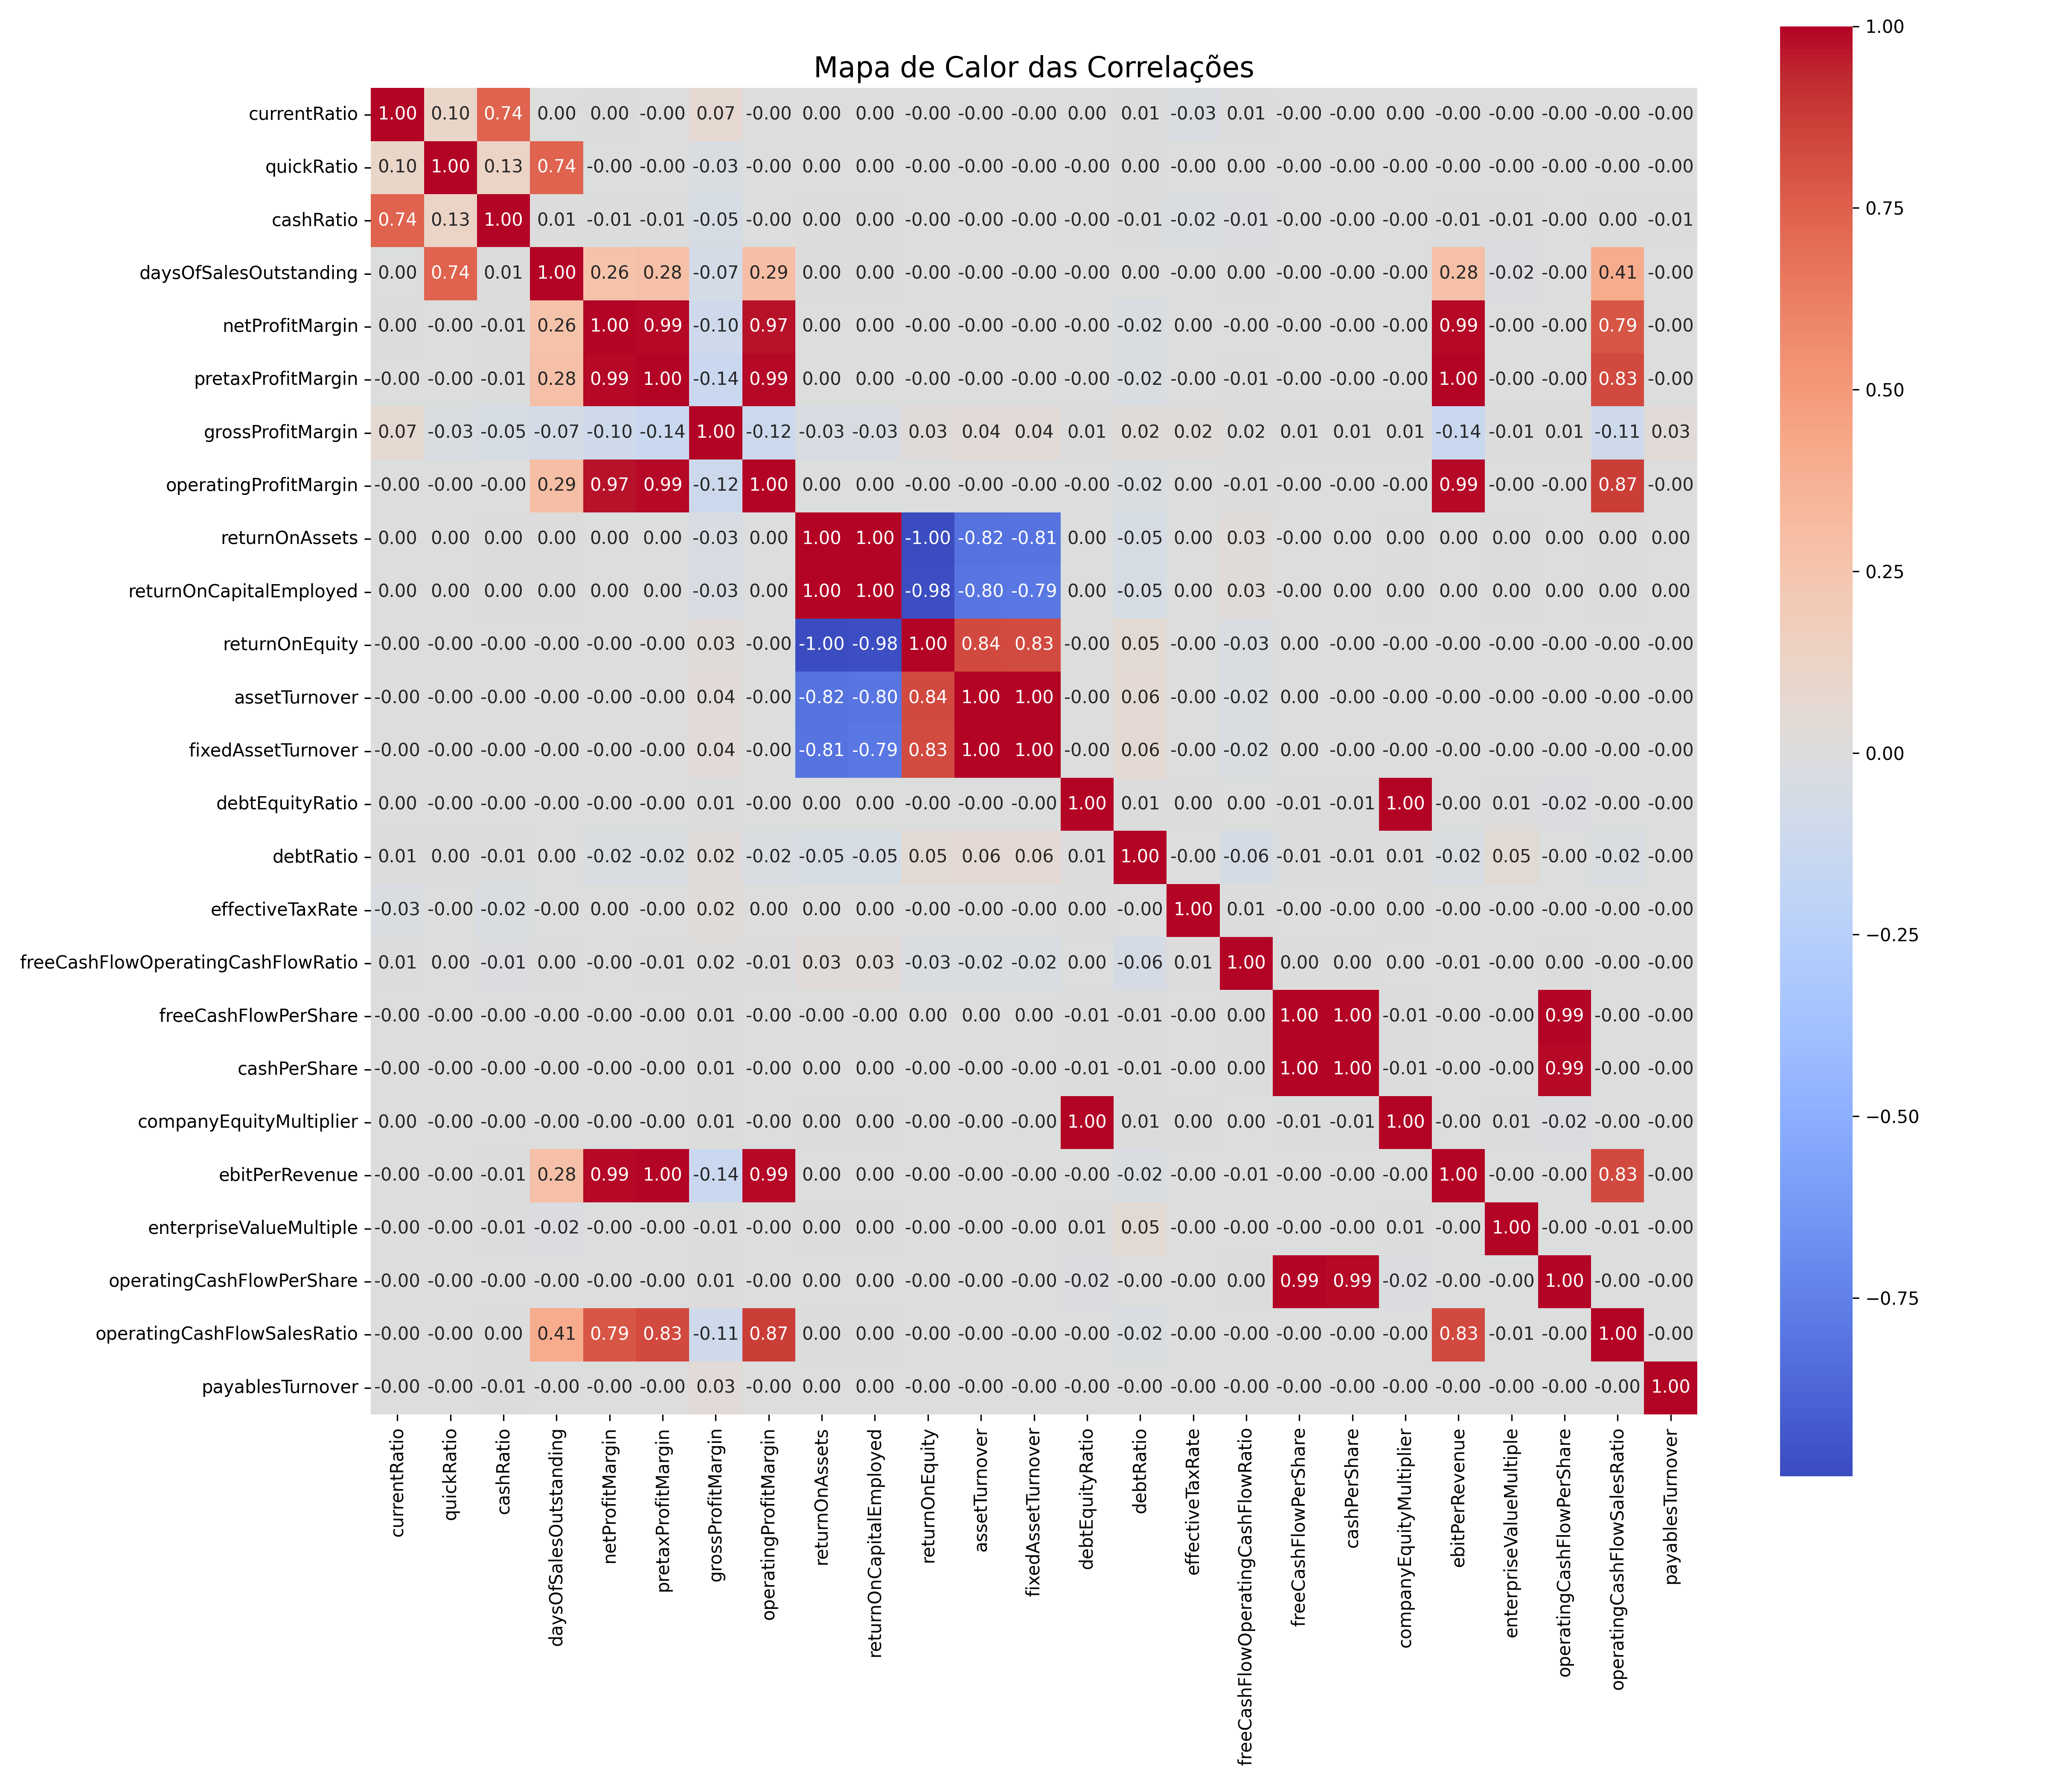
\includegraphics[width=0.85\textwidth]{figs/matriz_correlacao_inadimplencia.png}
    \caption{Matriz de correlação das variáveis do dataset \textit{Default of Credit Card Clients}.}
    \label{fig:matriz_correlacao_inadimplencia}
\end{figure}

A partir da matriz de correlação apresentada na Figura~\ref{fig:matriz_correlacao_inadimplencia}, é possível observar que as variáveis \texttt{BILL\_AMT1}, \texttt{BILL\_AMT2}, \texttt{BILL\_AMT3}, \texttt{BILL\_AMT4}, \texttt{BILL\_AMT5} e \texttt{BILL\_AMT6} possuem forte correlação entre si, caracterizando-se como colineares. Além disso, percebe-se que a variável \texttt{PAY\_5} apresenta forte correlação com \texttt{PAY\_4} e \texttt{PAY\_6}.

\subsection{Corporate Credit Rating}

O \textit{Corporate Credit Rating Dataset}, disponível no Kaggle \footnote{\url{https://www.kaggle.com/datasets/agewerc/corporate-credit-rating}}, contém 2029 registros e 31 variáveis, com dados financeiros de grandes empresas americanas listadas na NYSE e na Nasdaq entre 2010 e 2016. Destas, 30 são variáveis preditoras e uma é a variável alvo, correspondente à classificação de crédito atribuída às empresas. O conjunto inclui indicadores de liquidez, lucratividade, endividamento, fluxo de caixa e dados cadastrais, sendo utilizado para prever ratings de crédito — classificações emitidas por agências que indicam o risco de inadimplência das companhias.

As variáveis preditoras podem ser agrupadas da seguinte forma:

\begin{sloppypar}
\begin{itemize}
    \item \textbf{Índices de Liquidez:} \texttt{currentRatio}, \texttt{quickRatio}, \texttt{cashRatio}, \texttt{daysOfSalesOutstanding};
    \item \textbf{Indicadores de Lucratividade:} \texttt{grossProfitMargin}, \texttt{operatingProfitMargin}, \texttt{pretaxProfitMargin}, \texttt{netProfitMargin}, \texttt{effectiveTaxRate}, \texttt{returnOnAssets}, \texttt{returnOnEquity}, \texttt{returnOnCapitalEmployed};
    \item \textbf{Índices de Endividamento:} \texttt{debtRatio}, \texttt{debtEquityRatio};
    \item \textbf{Indicador de Desempenho Operacional:} \texttt{assetTurnover};
    \item \textbf{Indicadores de Fluxo de Caixa:} \texttt{operatingCashFlowPerShare}, \texttt{freeCashFlowPerShare}, \texttt{cashPerShare}, \texttt{operatingCashFlowSalesRatio}, \texttt{freeCashFlowOperatingCashFlowRatio}
\end{itemize}
A variável alvo, \texttt{Rating}, representa a classificação de crédito das empresas. Observa-se que esta variável está desbalanceada, com concentração significativa em poucas classes, especialmente nas categorias \textbf{BBB}, \textbf{BB} e \textbf{A}, que juntas correspondem a mais de 75\% dos registros. A Tabela~\ref{tab:dist_rating} apresenta a distribuição detalhada da variável alvo.
\end{sloppypar}

\begin{table}[H]
\centering
\caption{Distribuição da variável alvo (\texttt{Rating}) no dataset \textit{Corporate Credit Rating Dataset}}
\label{tab:dist_rating}
\begin{tabular}{lcc}
\hline
\textbf{Rating} & \textbf{Quantidade} & \textbf{Frequência (\%)} \\
\hline
BBB   & 671 & 33.07 \\
BB    & 490 & 24.15 \\
A     & 398 & 19.62 \\
B     & 302 & 14.88 \\
AA    & 89  & 4.39  \\
CCC   & 64  & 3.15  \\
AAA   & 7   & 0.34  \\
CC    & 5   & 0.25  \\
C     & 2   & 0.10  \\
D     & 1   & 0.05  \\
\hline
\textbf{Total} & 2029 & 100.00 \\
\hline
\end{tabular}
\end{table}

A seguir na Figura~\ref{fig:matriz_correlacao_corporate_credit_rating}, apresenta-se a matriz de correlação entre as variáveis do dataset:

\begin{figure}[H]
    \centering
    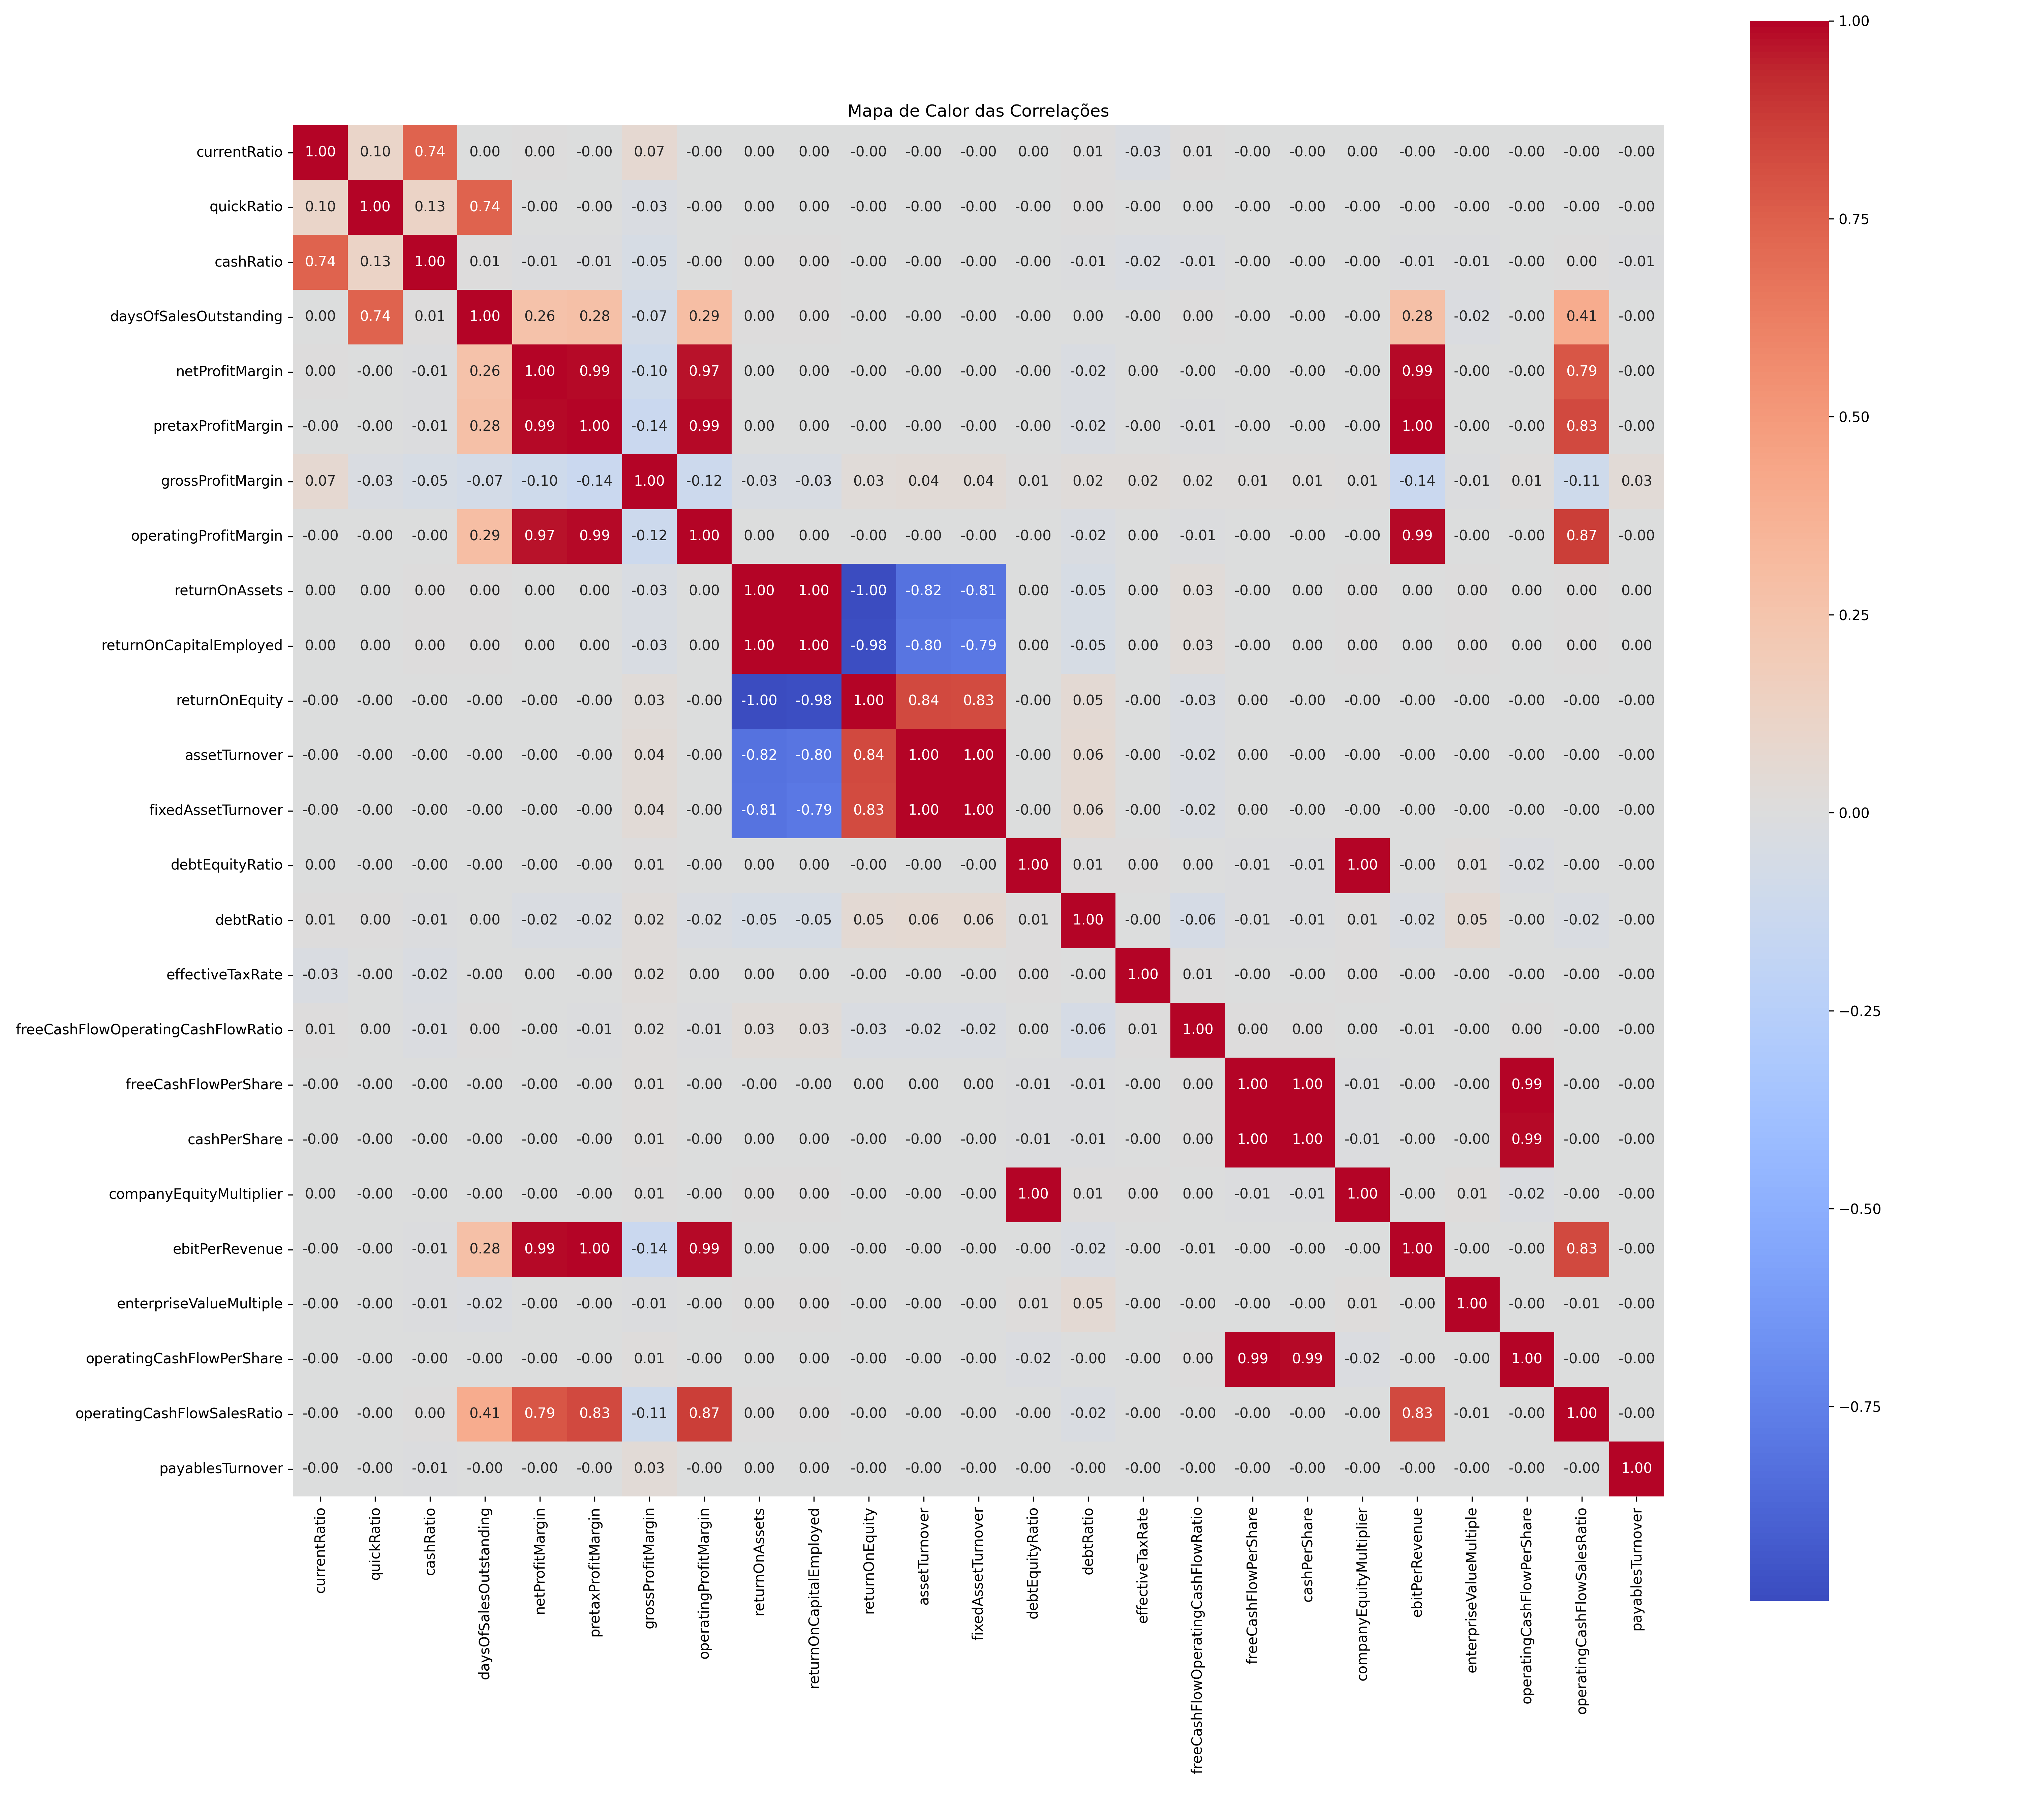
\includegraphics[width=0.85\textwidth]{figs/Correlacoes_Corporate_Credit_Rating.png}
    \caption{Matriz de correlação das variáveis do dataset \textit{Corporate Credit Rating Dataset}.}
    \label{fig:matriz_correlacao_corporate_credit_rating}
\end{figure}


\begin{sloppypar}
A partir da matriz de correlação apresentada na Figura~\ref{fig:matriz_correlacao_corporate_credit_rating}, observa-se colinearidade entre boa parte das variáveis. Destacam-se as variáveis \texttt{netProfitMargin}, \texttt{pretaxProfitMargin}, \texttt{grossProfitMargin}, \texttt{operatingProfitMargin}, \texttt{returnOnAssets}, \texttt{returnOnCapitalEmployed}, \texttt{returnOnEquity}, \texttt{assetTurnover}, \texttt{fixedAssetTurnover}, \texttt{debtEquityRatio}, \texttt{freeCashFlowPerShare}, \texttt{cashPerShare}, \texttt{companyEquityMultiplier}, \texttt{ebitPerRevenue}, \texttt{operatingCashFlowPerShare} e \texttt{operatingCashFlowSalesRatio}, que possuem correlação maior ou igual a 0,8 com uma ou mais variáveis preditoras.
\end{sloppypar}


\subsection{Conjunto de dados sintéticos}
Assim como em \citeonline{Salih2025AdditiveEffects}, o conjunto de dados sintético foi gerado utilizando o método \texttt{make\_classification} da biblioteca Scikit-learn, com os mesmos parâmetros utilizados no trabalho citado. Foram geradas 100 mil amostras com 16 variáveis preditoras (todas numéricas), nomeadas de \texttt{f1} a \texttt{f16}, das quais nove são informativas, cinco redundantes e duas representam ruído. Para introduzir diferentes níveis de colinearidade, foram adicionadas quatro novas variáveis (\texttt{f17}, \texttt{f18}, \texttt{f19} e \texttt{f20}) como combinações lineares de \texttt{f1}, \texttt{f2}, \texttt{f3} e \texttt{f4}, respectivamente.A variável alvo é balanceada e apresenta apenas duas classes, 0 ou 1.

A Figura~\ref{fig:matriz_correlacao_dados_sinteticos} apresenta matriz de correlação dos dados:

\begin{figure}[H]
    \centering
    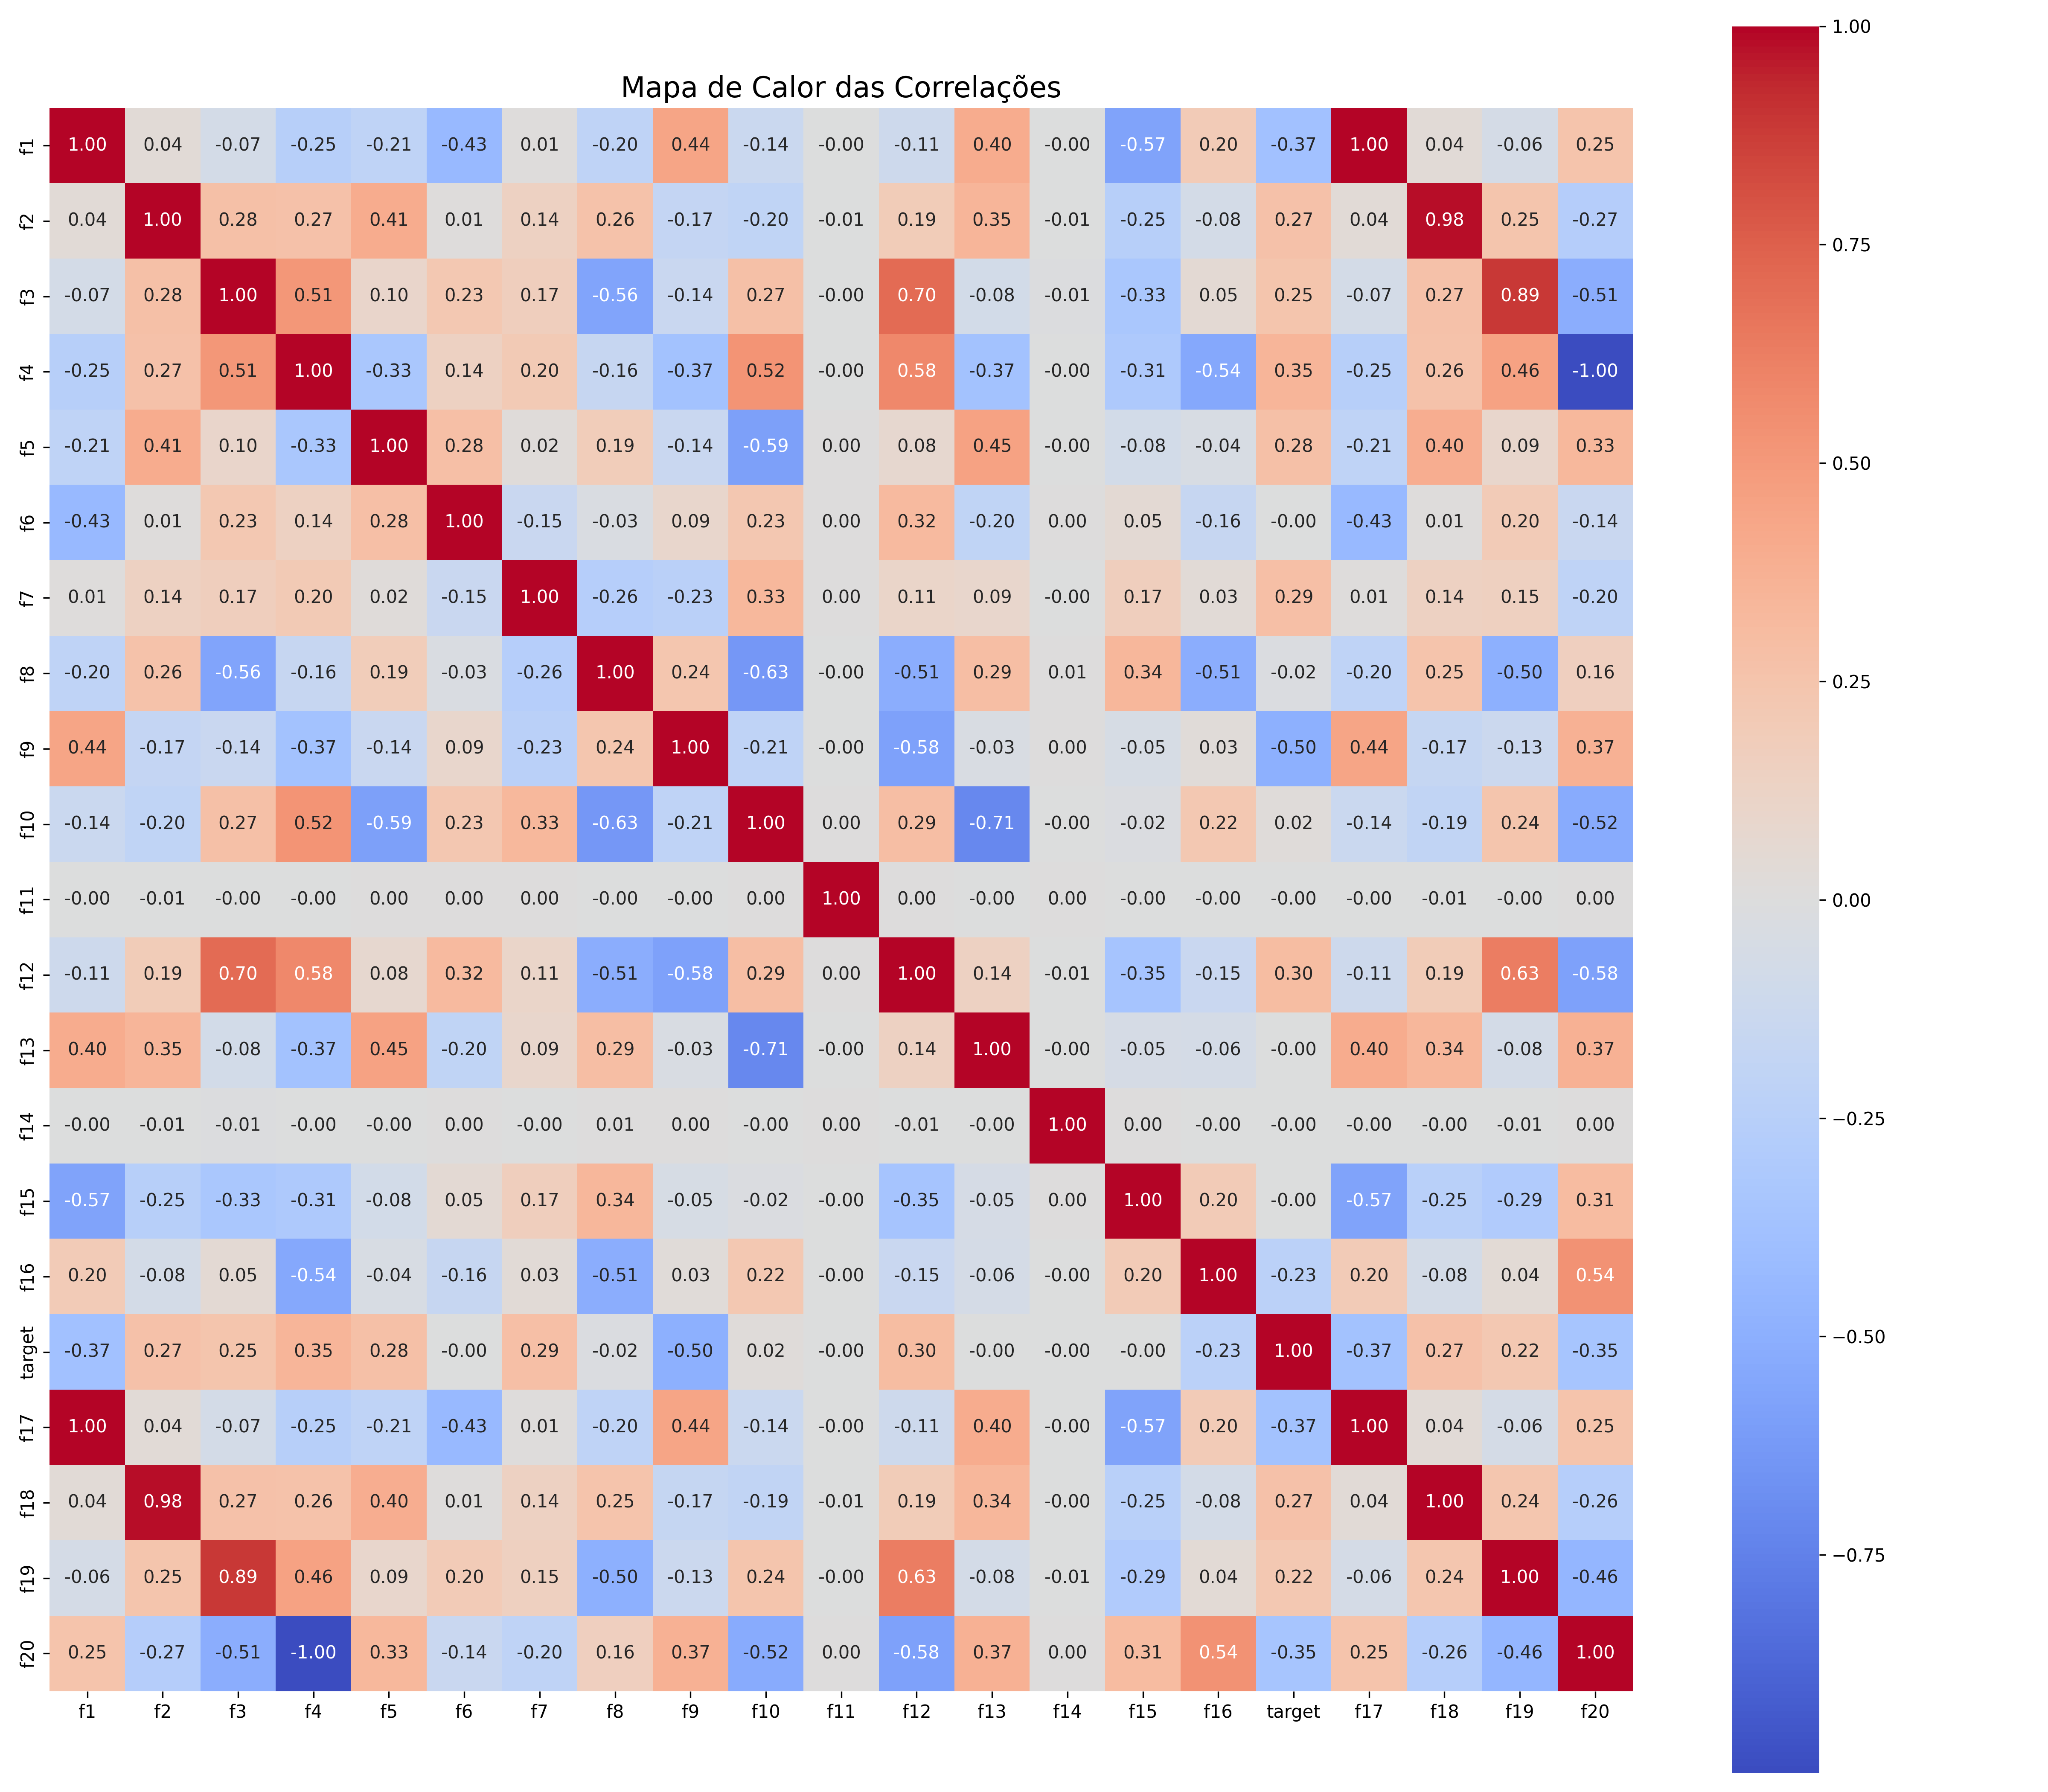
\includegraphics[width=0.85\textwidth]{figs/matriz_correlacao_dados_sinteticos.png}
    \caption{Matriz de correlação das variáveis do conjunto de dados sintéticos.}
    \label{fig:matriz_correlacao_dados_sinteticos}
\end{figure}


\section{Configuração do experimento}\label{sec:cofiguracao_experimentos}
Os conjuntos de dados serão divididos em dados de treino (70\%) e teste (30\%). Para cada conjunto, serão treinados e avaliados quatro algoritmos de classificação: SVM, Random Forest, LightGBM e XGBoost. Esses algoritmos foram escolhidos por serem amplamente utilizados, não serem naturalmente explicáveis e atenderem às limitações de recursos computacionais disponíveis para este trabalho. A implementação será realizada com a biblioteca Scikit-learn \cite{scikit-learn}, utilizando inicialmente os parâmetros padrão de cada modelo.

O desempenho preditivo dos algoritmos será avaliado com as métricas F1-score e Acurácia Balanceada, também disponíveis na biblioteca Scikit-learn. Essas métricas permitem uma avaliação equilibrada do desempenho geral do modelo, sem penalizar excessivamente falsos negativos ou falsos positivos. Após o treinamento e avaliação, serão aplicadas as técnicas SHAP e LIME, por meio das bibliotecas shap \footnote{\url{https://shap.readthedocs.io/en/latest/}} e lime \footnote{\url{https://lime-ml.readthedocs.io/en/latest/}}, respectivamente, para gerar explicações sobre as decisões dos modelos. A estabilidade das explicações será avaliada por meio da métrica NMR (\textit{Normalized Movement Rate}).

Posteriormente, o experimento será repetido utilizando dados transformados por PCA e dados com variáveis redundantes removidas, permitindo comparar o impacto da colinearidade na estabilidade das explicações geradas.


\section{Cronograma Geral}\label{sec:cronograma}

A Figura~\ref{fig:cronograma_geral} apresenta o cronograma geral para a realização deste trabalho. Cada PGC é dividido em quatro partes, e cada parte possui duração de três semanas.

\begin{figure}[htbp]
	\centering
	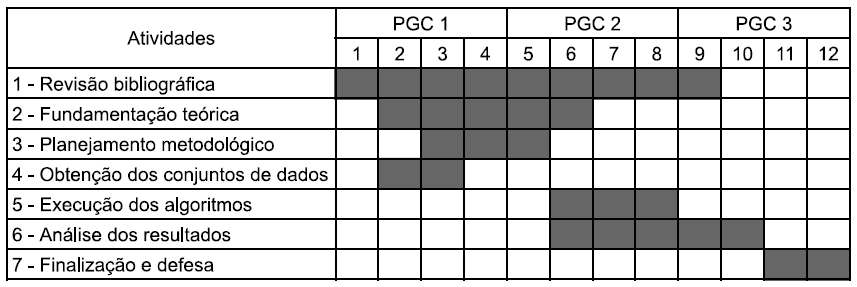
\includegraphics[width=0.85\textwidth]{figs/Cronograma_Pgc1.png}
	\caption{Cronograma geral da realização do trabalho.}
	\label{fig:cronograma_geral}
\end{figure}


A seguir, são descritas as principais etapas que compõem o desenvolvimento deste trabalho:
\begin{sloppypar}
\begin{enumerate}
	\item \textbf{Revisão bibliográfica:} consiste na busca, seleção e análise de artigos, livros e outras fontes acadêmicas relevantes, com o objetivo de mapear o estado da arte sobre o tema estudado e identificar lacunas de pesquisa.
	
	\item \textbf{Fundamentação teórica:} construção da base conceitual necessária para embasar o trabalho, apresentando as principais teorias, métodos e definições relacionadas ao tema.

	
	\item \textbf{Planejamento metodológico:} definição da abordagem de pesquisa, técnicas estatísticas e computacionais utilizadas, bem como a descrição dos procedimentos experimentais que serão adotados.
	
	\item \textbf{Obtenção dos conjuntos de dados:} etapa de coleta dos dados que serão utilizados nos experimentos.
	
	\item \textbf{Execução dos algoritmos:} aplicação prática dos modelos de aprendizado de máquina e de inteligência artificial explicável selecionados, contemplando o treinamento, validação e teste com os conjuntos de dados definidos.
	
	\item \textbf{Análise dos resultados:} interpretação dos resultados obtidos, comparando o desempenho dos modelos, avaliando métricas e discutindo os impactos da colinearidade sobre a estabilidade das explicações.
	
	\item \textbf{Finalização e defesa:} etapa de consolidação do trabalho, preparação da apresentação e defesa perante a banca examinadora.
\end{enumerate}
\end{sloppypar}


